\section{\textbf{Analysis of In-Domain Text}}

%%%%%%%%%%%%%%%%%%%%%%%%%%%%%%%%%%%%%%%%%%%%%%%%%%%%%%%%%%%%%%%%%%%%%%%%%%%%%%%%
\subsection{\textbf{Perplexity values}}

\begin{table}[ht]  %table 里面也可以嵌套tabular,只有tabular是不能加标题的
\centering  %表格居中
\caption{In-Domain Perplexity of the test set}
\begin{tabular}{lccc}
\hline
&    \textbf{Trigram + Smoothing} & \textbf{Trigram} & \textbf{Unigram} \\
\hline
 \textbf{Brown}   & 2619.47 &  18215.20 &  \textbf{1604.20}   \\
 \textbf{Reuters} &  \textbf{181.48} &  607.16  &  1500.69   \\
 \textbf{Gutenberg} & \textbf{390.65} & 1423.66 &  1005.79   \\
\hline
\end{tabular}
\label{tab:in-domain}
\end{table}

The computed perplexity of the test for three different corpus and the compared performance with baseline models is shown in Table~\ref{tab:in-domain}. As we can see, Trigram with Smoothing Technique outperforms Trigram on all three corpus, which suggests that our smoothing technique works! Furthermore, Trigram with Smoothing Technique also outperforms Unigram on Reuters and Gutenberg corpus. There is an interesting fact that Unigram outperforms Trigram with Smoothing Technique on Brown corpus. It may due to the relatively \textit{small} size of training data and \textit{huge} size of vocabulary. 

\begin{table}[ht]  %table 里面也可以嵌套tabular,只有tabular是不能加标题的
\centering  %表格居中
\caption{Dataset Distribution}
\begin{tabular}{lcccc}
\hline
&    \textbf{Train} & \textbf{Dev} & \textbf{Test} & \textbf{Vocab} \\
\hline
 \textbf{Brown}   & 39802 &  8437 & 8533 & \textbf{41746}   \\
 \textbf{Reuters} &  38169 &  8082  &  8214 & 36037   \\
 \textbf{Gutenberg} & \textbf{68740} & \textbf{14729} &  \textbf{14826} & \textbf{43835} \\
\hline
\end{tabular}
\label{tab:data_dis}
\end{table}

Next, We observe the trend when the amount of training data is varied. The results are shown in the figure~\ref{fig:ratio}. As we can see from the figure, performances of both Brown and Reuters increases as the data size increases, while the performance of Gutenberg seems to have a convergency when the ratio is approaching $1$. This makes sense since as Table~\ref{tab:data_dis} shows, Gutenberg is the largest among the three corpus. The phenomenon provides us with some insights to increase the model performance.

\begin{figure}[h]
\caption{Perplexity-Ratio Graph of dev set for different corpus}
\centering
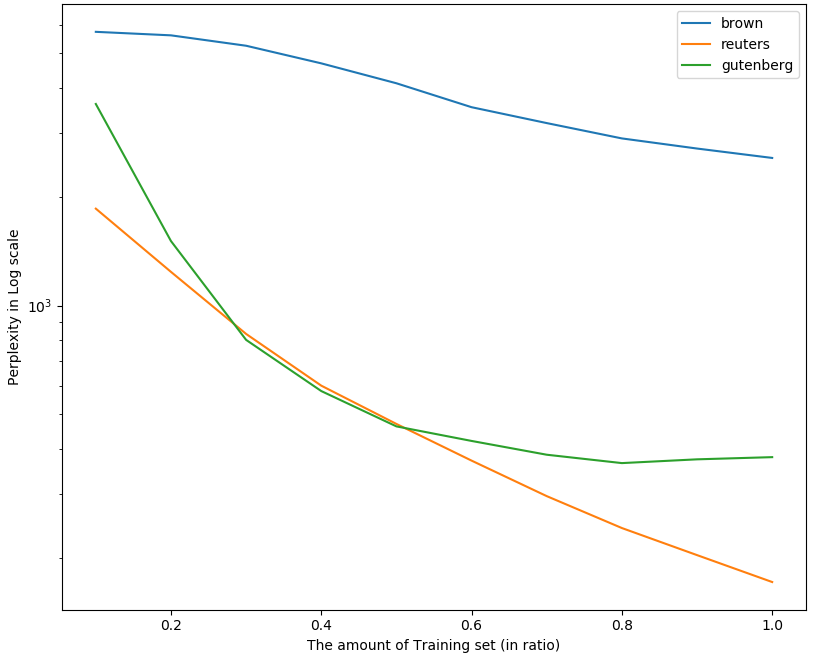
\includegraphics[width=0.45\textwidth]{files/figs/Perplexity-Ratio.png}
\label{fig:ratio}
\end{figure}



%%%%%%%%%%%%%%%%%%%%%%%%%%%%%%%%%%%%%%%%%%%%%%%%%%%%%%%%%%%%%%%%%%%%%%%%%%%%%%%%
\subsection{\textbf{Some Examples of sampled sentences}}

We generate samples using prefix \textit{To be or}. As we can see from the following results, the Unigram merely outputs some frequent words but makes nonsense. For Trigram models, however, whether with smoothing techniques or without, although the generated sentence may not make sense completely, there still are some \textit{local sense}, for example, the underlined expressions in the sentences do make sense.

Moreover, we can see the differences in the domain of training data can lead to the differences in the outputs of language models. For example, the outputs of Reuters is more related to financial domain.

\subsubsection{\textbf{Unigram}}

\begin{itemize}
\item Brown: \textit{To be or to at savings think Sarah and father to where and platform face...}
\item Reuters: \textit{To be or to is it supply chairman oil sources off affect losing letter...}
\item Gutenberg: \textit{To be or to whom}
\end{itemize}

\subsubsection{\textbf{Trigram without Smoothing}}

\begin{itemize}
\item Brown: \textit{To be or to \uline{put down on schedule}}
\item Reuters: \textit{To be or to \uline{hold oil prices} to \uline{farmers who have built several} Bertone X1 \uline{sports cars with structures}...}
\item Gutenberg: \textit{To be or \uline{to be baffled To manual work} for Ahab \uline{and also concerning the kingdom of God for he shall cause their terror}...}
\end{itemize}

\subsubsection{\textbf{Trigram with Smoothing}}

\begin{itemize}
\item Brown: \textit{To be or \uline{to costly improvements wedge} microorganisms 196 Means tumbles juniors interposed...}
\item Reuters: \textit{To be or to \uline{first quarter will have competitive advantage}...}
\item Gutenberg: \textit{To be \uline{or to rest with} antics fisher snug Expand hypocrites...}
\end{itemize}